\documentclass[journal,12pt,onecolumn]{IEEEtran}
\usepackage{cite}
\usepackage{graphicx}
\usepackage{amsmath,amssymb,amsfonts,amsthm}
\usepackage{algorithmic}
\usepackage{graphicx}
\usepackage{textcomp}
\usepackage{xcolor}
\usepackage{txfonts}
\usepackage{listings}
\usepackage{enumitem}
\usepackage{mathtools}
\usepackage{gensymb}
\usepackage{comment}
\usepackage[breaklinks=true]{hyperref}
\usepackage{tkz-euclide} 
\usepackage{listings}
\usepackage{gvv}                                        
\usepackage[latin1]{inputenc} 
\usetikzlibrary{arrows.meta, positioning}
\usepackage{xparse}
\usepackage{color}                                            
\usepackage{array}                                            
\usepackage{longtable}                                       
\usepackage{calc}                                             
\usepackage{multirow}
\usepackage{multicol}
\usepackage{hhline}                                           
\usepackage{ifthen}                                           
\usepackage{lscape}
\usepackage{tabularx}
\usepackage{array}
\usepackage{float}
\newtheorem{theorem}{Theorem}[section]
\newtheorem{problem}{Problem}
\newtheorem{proposition}{Proposition}[section]
\newtheorem{lemma}{Lemma}[section]
\newtheorem{corollary}[theorem]{Corollary}
\newtheorem{example}{Example}[section]
\newtheorem{definition}[problem]{Definition}
\newcommand{\BEQA}{\begin{eqnarray}}
\newcommand{\EEQA}{\end{eqnarray}}
\usepackage{float}
\theoremstyle{remark}
\usepackage{circuitikz}
\usepackage{tikz}
\title{GG: GEOLOGY AND GEOPHYSICS}
\author{EE25BTECH11032- KARTIK LAHOTI}

\begin{document}
\maketitle

\begin{enumerate}

\centering\section*{General Aptitude - GA }

\subsection*{Q.1. - Q.5 Multiple Choice Question (MCQ), carry ONE mark each(for each wrong answer: -1/3).}
    
    \item The people \rule{3cm}{0.15mm} were at the demonstration were from all sections of society. \hfill{\brak{\text{GATE GG 2021}}}
        \begin{enumerate}
            \begin{multicols}{4}               
                \item whose
                \item which
                \item who
                \item whom
            \end{multicols}
        \end{enumerate}
    
    \item A transparent square sheet shown above is folded along the dotted line. The folded sheet will look like \rule{3cm}{0.15mm}.\hfill{\brak{\text{GATE GG 2021}}}
        \begin{figure}[h]
            \centering            
            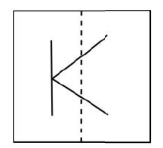
\includegraphics[width=0.2\columnwidth]{Figs/fig_1.png}
            \caption{Q.2.}
            \label{fig:q2}
        \end{figure}
    
    \begin{enumerate}
        \begin{multicols}{2}
            \item 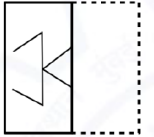
\includegraphics[width=0.4\columnwidth]{Figs/fig_1.1.png}
            \item 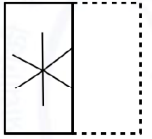
\includegraphics[width=0.4\columnwidth]{Figs/fig_1.2.png}
            \item 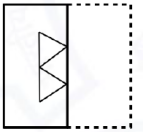
\includegraphics[width=0.4\columnwidth]{Figs/fig_1.3.png}
            \item 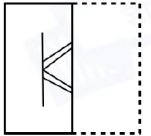
\includegraphics[width=0.4\columnwidth]{Figs/fig_1.4.png}
        \end{multicols}
    \end{enumerate}
    
    \item For a regular polygon having $10$ sides, the interior angle between the sides of the polygon, in degrees, is: \hfill{\brak{\text{GATE GG 2021}}}
        \begin{enumerate}
            \begin{multicols}{4}
                \item $396$
                \item $324$
                \item $216$
                \item $144$
            \end{multicols}
        \end{enumerate}
    
    \item Which one of the following numbers is exactly divisible by $\brak{11^{13}+1}$? \hfill{\brak{\text{GATE GG 2021}}}
        \begin{enumerate}
            \begin{multicols}{4}
                \item $11^{26}+1$
                \item $11^{33}+1$
                \item $11^{39}-1$
                \item $11^{52}-1$
            \end{multicols}
        \end{enumerate}
    
    \item Oasis is to sand as island is to \rule{3cm}{0.15mm} Which one of the following options maintains a similar logical relation in the above sentence? \hfill{\brak{\text{GATE GG 2021}}}
        \begin{enumerate}
            \begin{multicols}{4}
                \item Stone
                \item Land
                \item Water
                \item Mountain
            \end{multicols}
        \end{enumerate}
    
    \subsection*{Q.6. - Q.10. Multiple Choice Question (MCQ), carry TWO marks each (for each wrong answer: -2/3).}
    
    \item The importance of sleep is often overlooked by students when they are preparing for exams. Research has consistently shown that sleep deprivation greatly reduces the ability to recall the material learnt. Hence, cutting down on sleep to study longer hours can be counterproductive. Which one of the following statements is the CORRECT inference from the above passage?\hfill{\brak{\text{GATE GG 2021}}}
        \begin{enumerate}
            \item Sleeping well alone is enough to prepare for an exam. Studying has lesser benefit.
            \item Students are efficient and are not wrong in thinking that sleep is a waste of time.
            \item If a student is extremely well prepared for an exam, he needs little or no sleep.
            \item To do well in an exam, adequate sleep must be part of the preparation.
        \end{enumerate}
    
    \item In the figure shown above, each inside square is formed by joining the midpoints of the sides of the next larger square. The area of the smallest square \brak{\text{shaded}} as shown, in $cm^{2}$ is: \hfill{\brak{\text{GATE GG 2021}}}
        \begin{figure}[h]
            \centering
            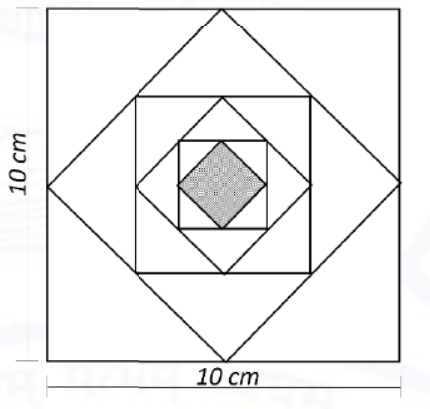
\includegraphics[width=0.4\columnwidth]{Figs/fig_2.png}
            \caption{Q.7.}
            \label{fig:q7}
        \end{figure}
    
        \begin{enumerate}
            \begin{multicols}{4}
                \item $12.50$
                \item $6.25$
                \item $3.125$
                \item $1.5625$
            \end{multicols}
        \end{enumerate}
    
    \item Let $X$ be a continuous random variable denoting the temperature measured. The range of temperature is [$0$, $100$] degree Celsius and let the probability density function of $X$ be $f\brak{x}=0.01 \text{for} 0 \leq X \leq 100$. The mean of $X$ is \rule{3cm}{0.15mm} \hfill{\brak{\text{GATE GG 2021}}}
        \begin{enumerate}
            \begin{multicols}{4}
                \item $2.5$
                \item $5.0$
                \item $25.0$
                \item $50.0$
            \end{multicols}
        \end{enumerate}
    
    \item The number of students passing or failing in an exam for a particular subject are presented in the bar chart above. Students who pass the exam cannot appear for the exam again. Students who fail the exam in the first attempt must appear for the exam in the following year. Students always pass the exam in their second attempt.
        \begin{figure}[h]
            \centering
            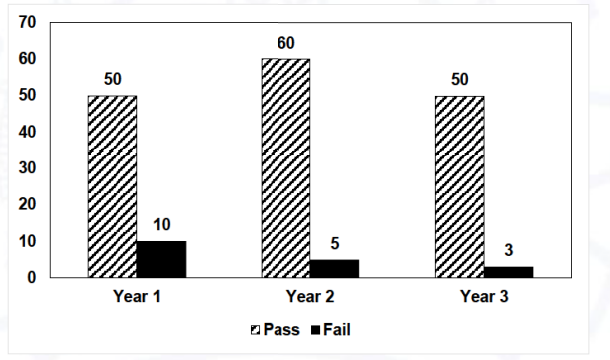
\includegraphics[width=0.6\columnwidth]{Figs/fig_3.png}
            \caption{Q.9.}
            \label{fig:q9}
        \end{figure}
    The number of students who took the exam for the first time in the year $2$ and the year $3$ respectively, are \rule{3cm}{0.15mm}. \hfill{\brak{\text{GATE GG 2021}}}
        \begin{enumerate}
            \begin{multicols}{4}
                \item $65\text{ and }53$
                \item $60\text{ and }50$
                \item $55\text{ and }53$
                \item $55\text{ and }48$
            \end{multicols}
        \end{enumerate}
    
    \item Seven cars P, Q, R, S, T, U and V are parked in a row not necessarily in that order. The cars T and U should be parked next to each other. The cars S and V also should be parked next to each other, whereas P and Q cannot be parked next to each other. Q and S must be parked next to each other. R is parked to the immediate right of V. T is parked to the left of U. Based on the above statements, the only INCORRECT option given below is: \hfill{\brak{\text{GATE GG 2021}}}
        \begin{enumerate}
            \item There are two cars parked in between Q and V.
            \item Q and R are not parked together.
            \item V is the only car parked in between S and R.
            \item Car P is parked at the extreme end.
        \end{enumerate}
    \end{enumerate}
\begin{center}
    \section*{\underline{Geophysics (GG)}}
\end{center}
    
\subsection*{Q.1. - Q.15 Multiple Choice Question (MCQ), carry ONE mark each (for each wrong answer: -1/3).}
    \begin{enumerate}
        
    \item Which of the given planets has the highest average density? \hfill{\brak{\text{GATE GG 2021}}}
        \begin{enumerate}
            \begin{multicols}{4}
                \item Mercury
                \item Venus
                \item Earth
                \item Mars
            \end{multicols}    
        \end{enumerate}
    
    \item In a multi-electrode resistivity tomography (ERT) survey, using equally spaced electrodes, which of the given configurations will provide the maximum number of data points?  \hfill{\brak{\text{GATE GG 2021}}}
        \begin{enumerate}
            \begin{multicols}{4} 
                \item Wenner array
                \item Axial Dipole-dipole array
                \item Axial Pole-dipole array
                \item Schlumberger array
            \end{multicols}            
        \end{enumerate}
    
    \item In Electromagnetic methods of prospecting, which one of the given options is CORRECT about frequency and type of current source for the Primary field used? \hfill{\brak{\text{GATE GG 2021}}}
        \begin{enumerate}
            \begin{multicols}{2}   
                \item High frequency A.C.
                \item Low frequency A.C.
                \item Both high frequency A.C. and D.C.
                \item Low frequency D.C.
            \end{multicols}            
        \end{enumerate}
    
    \item 'Group' is a unit of: \hfill{\brak{\text{GATE GG 2021}}}
            \begin{enumerate}
            \begin{multicols}{4}                
                \item Lithostratigraphy
                \item Sequence stratigraphy
                \item Biostratigraphy
                \item Chronostratigraphy
            \end{multicols}            
        \end{enumerate}
    
    \item Furongian is an Epoch of: \hfill{\brak{\text{GATE GG 2021}}}
        \begin{enumerate}
            \begin{multicols}{4} 
                \item Cambrian
                \item Ordovician
                \item Triassic
                \item Cretaceous
            \end{multicols}            
        \end{enumerate}
    
    \item The stage of textural maturity of a clay-rich sandstone containing poorly-sorted and angular framework grains is: \hfill{\brak{\text{GATE GG 2021}}}
        \begin{enumerate}
            \begin{multicols}{4}
                \item Mature
                \item Supermature
                \item Immature
                \item Submature    
            \end{multicols}
        \end{enumerate}
    
    \item Which one of the following structures indicates Synsedimentary deformation?\hfill{\brak{\text{GATE GG 2021}}}
        \begin{enumerate}
            \begin{multicols}{4}   
                \item Festoon bedding
                \item Flaser bedding
                \item Tabular bedding
                \item Convolute bedding
            \end{multicols}            
        \end{enumerate}
    
    \item Low value in SP log as observed in dispersed shales is mainly due to the impeded movement of: \hfill{\brak{\text{GATE GG 2021}}}
        \begin{enumerate}
            \begin{multicols}{4}
                \item $Na^{+}$
                \item $Cl^{-}$ ion
                \item $K^{+}$
                \item $OH^{-}$ ion
            \end{multicols}    
        \end{enumerate}
    
    \item In Radiometric survey, the $\gamma$-ray spectrometer count rate depends on: \hfill{\brak{\text{GATE GG 2021}}}
        \begin{enumerate}
            \item Cracks present in the target rock volume
            \item Solid angle of the target rock about the spectrometer
            \item Temperature in the target rock
            \item Pressure in the target rock
        \end{enumerate}
    
    \item The dimension of radiant emittance of a blackbody as per Stefan-Boltzmann law is:\hfill{\brak{\text{GATE GG 2021}}}
        \begin{enumerate}
            \begin{multicols}{4}
                \item $M^{0}L^{1}T^{-1}$
                \item $M^{1}L^{-1}T^{-2}$
                \item $M^{1}L^{2}T^{-2}$
                \item $M^{1}L^{0}T^{-3}$
            \end{multicols}            
        \end{enumerate}
    
    \item A surface geological process that can create a landform called Cirque is:\hfill{\brak{\text{GATE GG 2021}}}
        \begin{enumerate}
            \begin{multicols}{2}   
                \item aeolian deposition
                \item fluvial deposition
                \item glacial erosion
                \item deposition of volcanic ash
            \end{multicols}            
        \end{enumerate}
    
    \item If $\alpha\text{ and }\beta$ are P- and S-wave velocities, respectively, then $\alpha^{2}-\brak{4/3}\beta^{2}$ is equal to: $\brak{\kappa \text{ is the bulk modulus, } \mu \text{is shear modulus and } \rho \text{is density}}$ \hfill{\brak{\text{GATE GG 2021}}}
        \begin{enumerate}
            \begin{multicols}{4}
                \item $\kappa/\rho$
                \item $\mu/\rho$
                \item $\kappa+\mu/\rho$
                \item $\kappa-\mu/\rho$
            \end{multicols}
        \end{enumerate}
    
    \item Which one of the following phases is P-wave that converts to S-wave during passage through the solid inner core? \hfill{\brak{\text{GATE GG 2021}}}
        \begin{enumerate}
            \begin{multicols}{4} 
                \item PKIKP
                \item PKJKP
                \item PKhKP
                \item PKPPcP
            \end{multicols}                 
        \end{enumerate}
        
    \item In reduction of gravity data, the latitude correction is maximum at: \hfill{\brak{\text{GATE GG 2021}}}
        \begin{enumerate}
            \begin{multicols}{4}
                \item $35\degree$ latitude
                \item $45\degree$ latitude
                \item $55\degree$ latitude
                \item $65\degree$ latitude
            \end{multicols}
        \end{enumerate}
    
    \item The most coaliferous unit of the Gondwana Supergroup is: \hfill{\brak{\text{GATE GG 2021}}}
        \begin{enumerate}
            \begin{multicols}{2}
                \item Talchir Formation
                \item Barakar Formation
                \item Karharbari Formation
                \item Panchet Formation
            \end{multicols}
        \end{enumerate}
    
    \subsection*{Q.16. - Q.25 Numerical Answer Type (NAT), carry ONE mark each (no negative marks).}
    
    \item A vertical borehole encounters a shale bed of uniform thickness occurring at a depth of $5$ m and dipping $60\degree$. The borehole pierces through this shale bed for a length of $10\, m$ to reach a sandstone layer below. The true thickness of the shale bed is \rule{3cm}{0.15mm} $m$. [in integer] \hfill{\brak{\text{GATE GG 2021}}}
    
    \item The mass and volume of a fully dried soil sample are $2200\,gm$ and $1100\,cm^3$, respectively. If the specific gravity of the soil particles is $2.5$ and water density is $1\,gm/cm^3$, the void ratio of the soil is \rule{3cm}{0.15mm}. [round off to $2$ decimal places]\hfill{\brak{\text{GATE GG 2021}}}
    
    \item A constant-head permeability test was performed on a vertical sand column of height $40\,cm$ and cross-sectional area of $25\,cm^2$. During the test, when the loss of head was $50\,cm$, the volume of water collected in $2$ minutes was $300\,cm^3$. Applying Darcy's law, the calculated coefficient of permeability of the sand column is \rule{3cm}{0.15mm} $cm/sec$. [round off to $2$ decimal places] \hfill{\brak{\text{GATE GG 2021}}}
    
    \item The radius \brak{r} of the oblate spheroid at $45\degree$ latitude with ellipticity of polar flattening of $1/298.25$ and equatorial radius of $6378140\,m$ is \rule{3cm}{0.15mm} $km$. [round off to $2$ decimal places] \hfill{\brak{\text{GATE GG 2021}}}
    
    \item Light passes through two media with refractive indices of $1.75\text{ and }1.55$, respectively. The thickness of both the media is $30\,\mu m$. The resultant path difference of the yellow light component $\brak{\lambda = 589\,nm}$ is \rule{3cm}{0.15mm} $\mu m$. \hfill{\brak{\text{GATE GG 2021}}}
    
    \item The water table in an unconfined aquifer at a place near the coast is $1\,m$ above the Mean Sea Level. Given the densities of fresh and saline water as $1.001\text{ and }1.025 \,g/cc$ , respectively, the fresh-saline water interface at the same location should be at a depth of \rule{3cm}{0.15mm} $m$ from the water table. [round off to one decimal place] \hfill{\brak{\text{GATE GG 2021}}}
    
    \item The volume percentage of galena and quartz in an ore body of $Pb$ are $90\text{ and }10$, respectively. The densities of galena and quartz are $7.6\text{ and }2.65\,g/cc$ , respectively. The grade of the ore body in terms of weight percent of $Pb$ is \rule{3cm}{0.15mm}. $\brak{\text{Atomic weights of } Pb = 206 \text{ and } S=32}$ [round off to $2$ decimal places] \hfill{\brak{\text{GATE GG 2021}}}
    
    \item Normal moveout (NMO) for reflected phase of seismic data is $2$ milliseconds. Consider the diffraction source at the edge of the same reflector, where the shot point is now placed directly above diffraction source. In this case, the NMO due to diffraction is \rule{3cm}{0.15mm} milliseconds. [in integer] \hfill{\brak{\text{GATE GG 2021}}}
    
    \item In a $2D$ seismic survey, first receiver location is at $\brak{1000\, m , 4000\, m}$, second receiver location is at $\brak{2000\, m , 4000\, m}$ and the source location is at $\brak{2000\, m , 1000\, m}$. Consider P-wave velocity as $5000\, m/sec$. The difference in first arrival time of P-wave phase for the two receivers is \rule{3cm}{0.15mm} seconds. [round off to $2$ decimal places] \hfill{\brak{\text{GATE GG 2021}}}
    
    \item The potential difference measured between potential electrodes using Wenner array is $500\,mV$ when a current of $2\,A$ is passed through the subsurface between current electrodes. If the computed apparent resistivity is $100\,\ohm m$ then the distance between the current electrodes will be \rule{3cm}{0.15mm} $m$. [round off to $2$ decimal places] [Use $\pi=3.141$] \hfill{\brak{\text{GATE GG 2021}}}
    
    \subsection*{Q.26. - Q.42. Multiple Choice Question (MCQ), carry TWO marks each (for each wrong answer: -2/3).}
    
    \item In a horizontally stratified cuboid rock sample (stratified in vertical z direction with various layers of different resistivity), bulk resistivity is measured in three perpendicular directions. If $\rho_1, \rho_2\text{ and }\rho_3$ are the bulk resistivities measured perpendicular to $xy$, $xz$ and $yz$ planes, respectively, then
    
    \hfill{\brak{\text{GATE GG 2021}}}
        \begin{enumerate}
            \begin{multicols}{2}
                \item $\rho_1 < \rho_2 = \rho_3$
                \item $\rho_1 > \rho_2 = \rho_3$
                \item $\rho_1 = \rho_2 \ne \rho_3$
                \item $\rho_1 \ne \rho_2 \ne \rho_3$
            \end{multicols}
        \end{enumerate}
    
    \item Which one is the CORRECT sequence of electromagnetic methods in terms of depth of investigation? \\
    P - AFMAG method \\
    Q - VLF method \\
    R - GPR method \\
    S - Magnetotelluric method \hfill{\brak{\text{GATE GG 2021}}}
        \begin{enumerate}
            \begin{multicols}{2}
                \item P $>$ Q $>$ S $>$ R
                \item P $>$ S $>$ R $>$ Q
                \item S $>$ P $>$ Q $>$ R
                \item S $>$ Q $>$ R $>$ P
            \end{multicols}
        \end{enumerate}
    
    \item Which Norm gives the maximum weight to the data points having maximum deviation/outlier from the smoothly fitted curve during linearized inversion? \hfill{\brak{\text{GATE GG 2021}}}
        \begin{enumerate}
            \begin{multicols}{4}
                \item L$1$-Norm
                \item L$2$-Norm
                \item Lp-Norm
                \item L$\infty$-Norm
            \end{multicols}
        \end{enumerate}
    
    \item Which one of the following statements is CORRECT for the Quenching agent used in the tube of Geiger-Muller counter? \hfill{\brak{\text{GATE GG 2021}}}
        \begin{enumerate}
                \item It enhances the emission of secondary electrons from the cathode.
                \item It reduces the emission of secondary electrons from the cathode.
                \item It enhances the emission of secondary electrons from the anode.
                \item It reduces the emission of secondary electrons from the anode.
        \end{enumerate}
    
    \item Which one of the following statements is CORRECT regarding the property of Laplacian operator for vector/scalar fields? \hfill{\brak{\text{GATE GG 2021}}}
        \begin{enumerate}
            \item Laplacian of a vector field is zero if the Laplacian of each of its components are zero.
            \item Laplacian of a vector field is zero if the Laplacian of any one of its component is zero.
            \item If the Laplacian of a scalar field is zero then the scalar field is not harmonic.
            \item If the Laplacian of a scalar field is finite (non-zero) then the scalar field is harmonic.
        \end{enumerate}
    
    \item The most desirable interaction of $\gamma$-ray with matter for $\gamma$-ray spectroscopy is
    
    \hfill{\brak{\text{GATE GG 2021}}}
        \begin{enumerate}
                \item Photoelectric effect only
                \item Both Photoelectric effect and Compton scattering
                \item Both Compton Scattering and Pair production
                \item Photoelectric effect, Compton scattering and Pair production
        \end{enumerate}
    
    \item Which one of the following is the CORRECT sequence for a $2D$ seismic reflection data processing prior to Time-depth conversion? \hfill{\brak{\text{GATE GG 2021}}}
        \begin{enumerate}
            \item Migration $\rightarrow$ Deconvolution $\rightarrow$ Filtering $\rightarrow$ Equalization $\rightarrow$ Coherency
            \item Deconvolution $\rightarrow$ Migration $\rightarrow$ Filtering $\rightarrow$ Coherency $\rightarrow$ Equalization
            \item Filtering $\rightarrow$ Deconvolution $\rightarrow$ Migration $\rightarrow$ Equalization $\rightarrow$ Coherency
            \item Deconvolution $\rightarrow$ Filtering $\rightarrow$ Equalization $\rightarrow$ Migration $\rightarrow$ Coherency
        \end{enumerate}
    
    \item Choose the CORRECT procedure to avoid the area of cracked, altered formation in Sonic log. \hfill{\brak{\text{GATE GG 2021}}}
        \begin{enumerate}
                \item Measure interval transit times using long-spacing sonic tools.
                \item Use more number of sets of sources.
                \item Measure interval transit times using short-spacing sonic tools.
                \item Use more number of sets of detectors.
        \end{enumerate}
    
    \item The factor that DOES NOT influence measurement of Nuclear Magnetic Resonance log is \hfill{\brak{\text{GATE GG 2021}}}
        \begin{enumerate}
		\begin{multicols}{2}
                	\item mineral composition of the rock
                	\item bound water (irreducible water).
                	\item free water.
                	\item pore fluid pressure.
		\end{multicols}	
        \end{enumerate}
    
    \item Consider a time-invariant geophysical filter with the given input as: $x(t) = e^{-\alpha t}$ when $t \ge 0$; $x(t) = 0$ when $t < 0$ and output $y(t) = e^{-\beta t}$ when $t \ge 0$; $y(t) = 0$ when $t < 0$. The transfer function for the given input and output of time-invariant filter will be: \hfill{\brak{\text{GATE GG 2021}}}
        \begin{enumerate}
            \begin{multicols}{4}   
                \item $\frac{\alpha + i\omega}{\beta - i\omega}$
                \item $\frac{\alpha + i\omega}{\beta + i\omega}$
                \item $\frac{\alpha - i\omega}{\beta + i\omega}$
                \item $\frac{\alpha - i\omega}{\beta - i\omega}$
            \end{multicols}
        \end{enumerate}
    
    \item Which of the given figures is the Hilbert transform of the Dirac delta function $\delta\brak{\xi}$: \hfill{\brak{\text{GATE GG 2021}}}
        \begin{figure}[h]
            \centering
            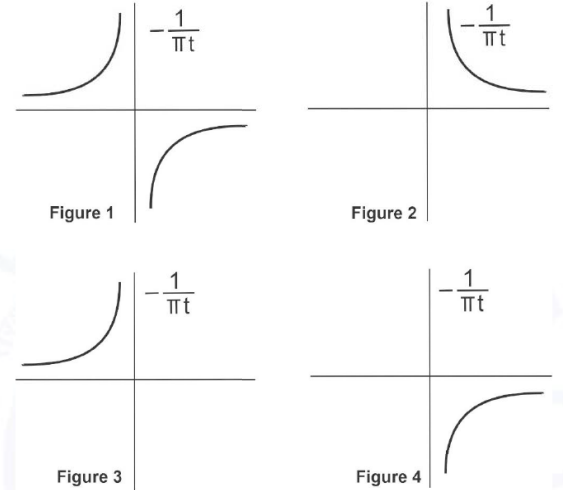
\includegraphics[width=0.5\columnwidth]{Figs/fig_4.png}
            \caption{Q.36.}
            \label{fig:q.36}
        \end{figure}
    
        \begin{enumerate}
            \begin{multicols}{4}
                \item Figure 1
                \item Figure 2
                \item Figure 3
                \item Figure 4
            \end{multicols}
        \end{enumerate}
    
    \item If a mountain range is $100\%$ isostatically compensated (Airy's type), what would be the expected nature of the Bouguer anomaly and free-air anomaly?\hfill{\brak{\text{GATE GG 2021}}}
        \begin{enumerate}
                \item Bouguer anomaly is very large and negative; free air anomaly is small and positive.
                \item Bouguer anomaly is very large and negative; free air anomaly is large and positive.
                \item Bouguer anomaly is exactly zero; free air anomaly is very large and positive.
                \item Bouguer anomaly is very large and negative; free air anomaly is large and negative.
        \end{enumerate}
    
    \item Which of the following is INCORRECT for a recorded nuclear explosion event? \hfill{\brak{\text{GATE GG 2021}}}
        \begin{enumerate}
            \item The first P-wave from an explosion source to arrive t any seismic station, irrespective of Azimuth, should be compressional.
            \item Nuclear explosions are not as good as earthquakes at generating surface waves or S-waves.
            \item In general, earthquakes have Mb values same those for nuclear explosions with same Ms values.
            \item Nuclear explosions have all been shallower than $2\,km$ depth.
        \end{enumerate}
    
    \item Focal depth can be determined from measurement of the difference in the travel time between: \hfill{\brak{\text{GATE GG 2021}}}
                \begin{enumerate}
                    \begin{multicols}{4}
                        \item pP and P
                        \item PP and P
                        \item PcP and P
                        \item PPP and P
                    \end{multicols}
                \end{enumerate}
    
    \item Of the following options, at which discontinuity both P-wave and S-wave have maximum velocity drop? \hfill{\brak{\text{GATE GG 2021}}}
                \begin{enumerate}
                    \begin{multicols}{4}
                        \item Conard
                        \item Mohorovicic
                        \item Gutenberg
                        \item Lehman
                    \end{multicols}
                \end{enumerate}
    
    \item In data enhancement techniques, what is the advantage of magnetic anomaly being 'Reduced to the pole'? \hfill{\brak{\text{GATE GG 2021}}}
                \begin{enumerate}
                        \item Enhances the signal to noise ratio.
                        \item Estimates the depth to the basement.
                        \item Takes care of variation of the magnetic anomaly with latitude.
                        \item Helps in pseudo-gravity transformation.
                \end{enumerate}
    
    \item Match the source in Group - $I$ with their half-width $\brak{X_{1/2}} / \delta g_{max}$ and depth $\brak{d}$ relation in Group - $II$ \hfill{\brak{\text{GATE GG 2021}}}
    
            \begin{multicols}{2}
                \underline{\textbf{Group $I$}}
                \begin{enumerate}[start =16]
                    \item Sphere
                    \item Horizontal Cylinder
                    \item Steeply dipping sheet
                    \item Irregular body
                \end{enumerate}
    
                \columnbreak
    
                \underline{\textbf{Group $II$}}
                \begin{enumerate}
                    \item $d = 0.7 X_{1/2}$
                    \item $d \leq 0.86 \times \brak{\frac{\delta g_{max}}{\brak{\frac{dg}{dx} }_{max}}}$
                    \item $d = 1.3 X_{1/2}$
                    \item $s = X_{1/2}$
                \end{enumerate}
            \end{multicols}
    
            \begin{enumerate}
                \begin{multicols}{2}        
                    \item P-$1$, Q-$2$, R-$4$, S-$3$
                    \item P-$1$, Q-$4$, R-$3$, S-$2$
                    \item P-$3$, Q-$4$, R-$1$, S-$2$
                    \item P-$3$, Q-$1$, R-$4$, S-$2$
                \end{multicols}                
            \end{enumerate}

\subsection*{Q.43. - Q.55 Numerical Answer Type (NAT), carry TWO mark each (no negative marks).}


    \item If a gravity determination is made at an elevation of $150\,m$ above mean sea level, the Bouguer correction required for a density contrast of $250\,kg/m^3$ with the surroundings is \rule{3cm}{0.15mm} $mgal$. [round off to $2$ decimal places] \hfill{\brak{\text{GATE GG 2021}}}
    
    \item An infinite horizontal cylinder of radius $40\,km$ is buried at a depth of $100\,km$ and yields the same maximum gravity anomaly as that of an infinite horizontal cylinder of radius $1\,km$, buried at a depth of $1\,km$ having density contrast with the surroundings of $200\,kgm^{-3}$. The density contrast of the deeper cylinder with respect to the surrounding is \rule{3cm}{0.15mm} $kg/m^3$. [round off to one decimal place]  \hfill{\brak{\text{GATE GG 2021}}}
    
    \item An earthquake causes an average of $25\,m$ strike slip displacement over a $50\,km$ long, $25\,km$ deep portion of a transform fault. Assuming that the rock rigidity is $3 \times 10^{10}\, Nm^{-2}$, the moment magnitude $\brak{Mw}$ of the earthquake is \rule{3cm}{0.15mm}. [round off to $2$ decimal places] \hfill{\brak{\text{GATE GG 2021}}}
    
    \item Lithological unit $X$ is sandwiched between $Y1$ above and $Y2$ below it. Now consider a log across lithology $X$, where Gamma ray (GR) reading is given by $100\,API$; $Y1$ lithology, where minimum GR reading is $10\,API$; and $Y2$ lithology of shale, where GR reading is $200\,API$. Then the shale-free fractional volume in the $X$ lithology will be \rule{3cm}{0.15mm}. [round off to $2$ decimal places] \hfill{\brak{\text{GATE GG 2021}}}
    
    \item In a $2D$ seismic survey, $25$ receivers are placed in a group and $25$ sources are placed in another group, where random noise is present. The signal to noise ratio for this arrangement will be \rule{3cm}{0.15mm}. [in integer]  \hfill{\brak{\text{GATE GG 2021}}}
    
    \item In a VSP survey, the tube wave passage through borehole causes cross-section area change from $0.79\,m^2 \text{ to } 1.13\,m^2$. The transmission coefficient will be \rule{3cm}{0.15mm}. [round off to $2$ decimal places]  \hfill{\brak{\text{GATE GG 2021}}}
    
    \item In a cratonic region, radioactive heat generation decreases exponentially with depth. Assuming characteristic depth as $10\,km$ and surface heat generation as $3\,\mu W m ^{-3}$ and neglecting mantle heat flow, the heat production per unit volume for a $30\,km$ thick layer will be \rule{3cm}{0.15mm} $\mu W m^{-3}$. [round off to $2$ decimal places] \hfill{\brak{\text{GATE GG 2021}}}
    
    \item In an Induced Polarization survey, $50$ milliseconds chargeability was measured for steady state voltage (full saturation reached) of $200\,V$ between potential electrodes. When the current was switched off, the voltage across potential electrodes drops instantaneously $\brak{\text{time } t = 0\,s}$ to a level Va and thereafter decays linearly with time and becomes zero in $10$ seconds. The magnitude of instantaneous voltage Va $\brak{\text{at time } t = 0\,s}$ will be \rule{3cm}{0.15mm} $mV$. [in integer] \hfill{\brak{\text{GATE GG 2021}}}
    
    \item Apparent resistivity sounding data for Schlumberger array is theoretically generated by the teacher for the following $4$-layer model as: $\rho_1 = 100 \Omega\,m, \rho_2 = 20 \Omega\,m, \rho_3 = 500 \Omega\,m, \rho_4 = 10 \Omega\,m$ and layer thicknesses $h_1 = 50\,m, h_2 = 20\,m and h_3 = 50\,m$. If the student interprets this theoretical sounding data for $\rho_3$ as $750\,\Omega m$, then according to the Principle of Equivalence, the thickness $h_3$ would be \rule{3cm}{0.15mm} $m$. [round off to $2$ decimal places] \hfill{\brak{\text{GATE GG 2021}}}
    
    \item A $3D$ conducting body is located at a depth of $50\,m$ in a homogeneous medium of resistivity $500\,\Omega\,m$. A frequency of $f_1\,Hz$ is appropriate to detect this conducting body in a plane wave EM survey. When the same conducting body is located in a host medium of resistivity $100\,\Omega\,m$ at the same depth then a frequency of $f_2\,Hz$ is found to be appropriate. Then the value of $\frac{f_2}{f_1}$ will be \rule{3cm}{0.15mm}. [round off to $2$ decimal places] \hfill{\brak{\text{GATE GG 2021}}}
    
    \item The apparent resistivity and phase computed for MT measurement at $10^{-3}\,Hz$ frequency is $500\,\Omega\,m \text{ and } 30\degree$, respectively. Ratio of Imaginary to Real component of the Impedance tensor is \rule{3cm}{0.15mm}. [round off to $2$ decimal places] \hfill{\brak{\text{GATE GG 2021}}}
    
    \item The diagonal elements of a covariance matrix computed for a linearized inverse problem having model parameters $m_1, m_2, m_3, m_4, m_5 \text{are} 49, 15, 3, 200, 40$, respectively. The standard deviation (uncertainty) in the estimation of model parameters $m_4$ is \rule{3cm}{0.15mm}. [round off to $2$ decimal places]\hfill{\brak{\text{GATE GG 2021}}}
    
    \item Electric current density incident at an angle $40\degree$ from vertical at the horizontal interface between two layers with resistivity $\rho_1 = 100\,\Omega\,m \text{and} \rho_2 = 500\,\Omega\,m$ (from layer 1 to layer 2). The current density will enter into the second layer at an angle \rule{3cm}{0.15mm} degrees from vertical. [round off to $2$ decimal places] \hfill{\brak{\text{GATE GG 2021}}}

\centering\subsection*{END OF THE QUESTION PAPER}
\end{enumerate}
\end{document}
